\chapter{Simulations} \label{chap-3}

Holmes et al. recently performed PIC simulations in the original ORBIT code to determine the feasibility of elliptical painting in the SNS \cite{Holmes2018}. Their findings are reviewed in this chapter. Additionally, the simulations are extended in PyORBIT to include updated experimental constraints. First, the computational model is briefly described. 


\section{Computational model}


\subsection{Single-particle tracking}

The PyORBIT code tracks a Bunch object containing a set of 6D phase space coordinates. The accelerator is modeled as a series of nodes, each of which modifies the coordinates in some way. The core of PyORBIT is comprised of single-particle tracking routines. The approach used is inspired by TEAPOT (Thin-Element Accelerator Program for Optics and Tracking), where particles pass through a series of drifts and "kicks" from thin elements — elements with infinitesimal length \cite{Schachinger1987}. Each drift changes the particle's position without changing its momentum, while each kick changes the particle's momentum without changing its position. Thick elements are then approximated as a series of thin elements connected with drifts. The momentum kicks are derived from the Hamiltonian of a charged particle in an electromagnetic field. It can be shown that for a Hamiltonian $H$ that does not explicitly depend on $s$ (the time-like variable), then over a distance $L$, a function $g$ of the canonical coordinates will transform as
%
\begin{equation}
    g \rightarrow 
    = e^{-L:H:} g
    = \sum_{n=0}^{\infty}{\frac{L^n}{n!} (-:H:)^n g},
\end{equation}
%
where the operator $:H:$ is defined by
%
\begin{equation}
    \{H, g\} \equiv \, :H: g =
    \frac{\partial{H}}{\partial{\mathbf{q}}}
    \cdot
    \frac{\partial{g}}{\partial{\mathbf{p}}}
    -
    \frac{\partial{H}}{\partial{\mathbf{p}}}
    \cdot
    \frac{\partial{g}}{\partial{\mathbf{q}}}
\end{equation}
%
[Ref: Holmes (forthcoming), Forest]. Symplectic maps connecting the initial and final phase space coordinates are derived for elements such as drifts, dipoles, quadrupoles, etc.

Fringe fields need to be taken into account for elements of finite length, that is, the fields outside the start and end of the element. For example, the magnetic field in a solenoid has a transverse component near the edges that vanishes in the limit of infinite length. [...] [Ref: Forest]. The strength of fringe fields generally increases with the distance off-axis, so they are especially important in the injection region.

Longitudinal dynamics have not yet been discussed. Longitudinal focusing in the SNS ring is provided by two RF cavities. The harmonic frequency $h$ is defined as the RF frequency divided by the revolution frequency of the beam; one cavity operates at $h = 1$ and the other operates at $h = 2$, both at an amplitude near 5 kV. The energy gain $\Delta \epsilon$ for a particle passing through the cavity is approximated as  
%
\begin{equation}\label{eq:RF}
    \Delta \epsilon = q V \sin(h \phi + \phi_0),
\end{equation}
%
where the particle phase $\phi$ is zero for the synchronous particle. Since particles see different accelerating voltages depending on their arrival time, they oscillate in a stable region of longitudinal phase space. Since two harmonics are used, there are two peaks in the distribution. The longitudinal tune is four orders of magnitude smaller than the transverse tune in the SNS ring. 



\subsection{Collective effects}

Collective effects are important for high-intensity applications, and their calculation is a major component of beam physics simulations. We focus first on space charge. PyORBIT uses the particle-in-cell (PIC) method in which an $N$ particle bunch is represented by $M$ macroparticles, where $M \ll N$. The macroparticles are tracked according to Eq.~\eqref{eq:eom_with_spacecharge}. The electric field is obtained by solving Eq.~\eqref{eq:Poisson} on a grid. The key step is transforming between the discrete and continuous representation. The PIC loop is shown in Fig.~\ref{fig:pic_loop}. 
%
\begin{figure}[!p]
    \centering
    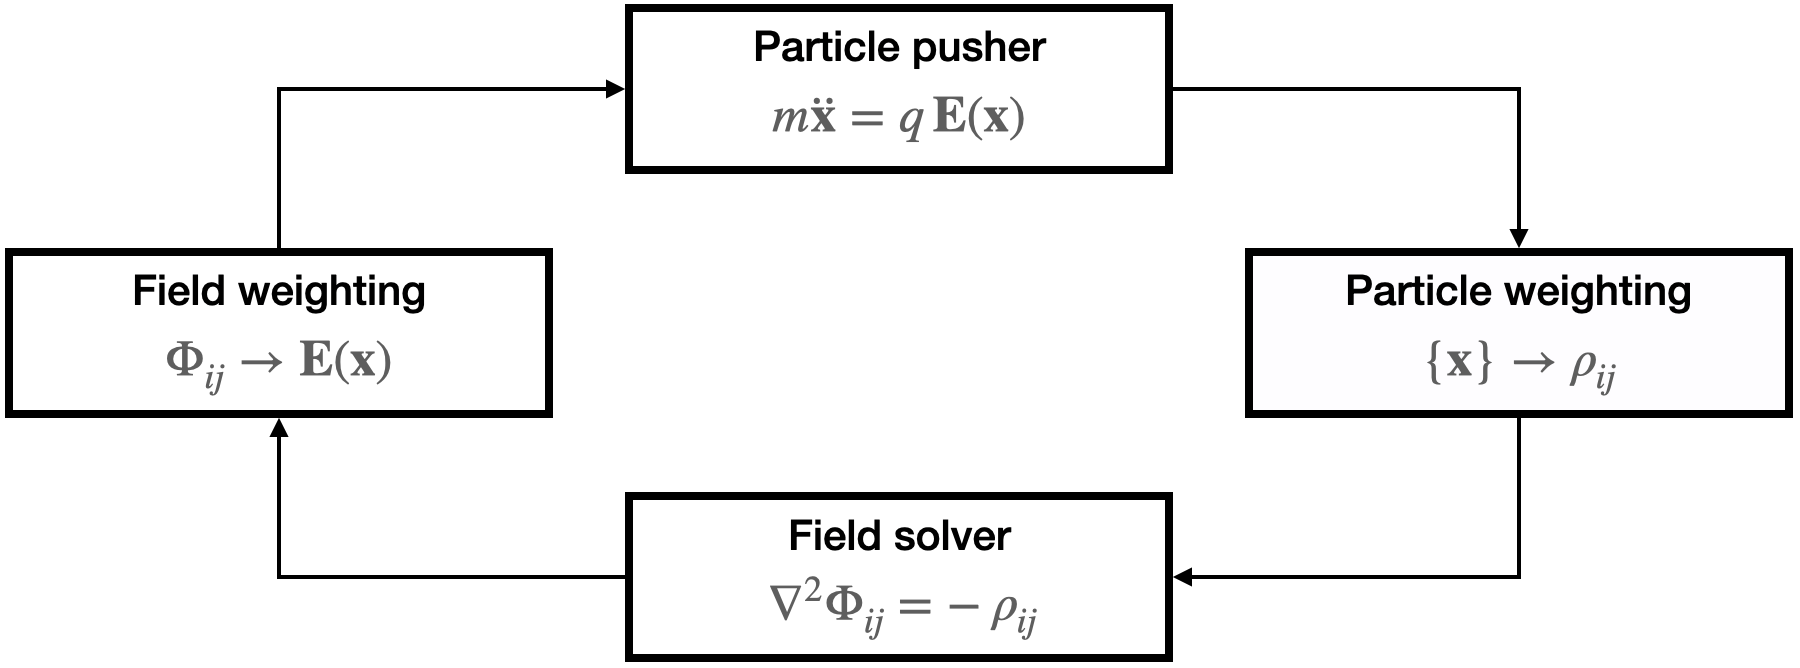
\includegraphics[width=\textwidth]{Images/chapter3/pic_loop.png}
    \caption{\label{fig:pic_loop}The particle-in-cell loop.}
    \vfill
    \vspace*{2.5cm}
    \vfill
    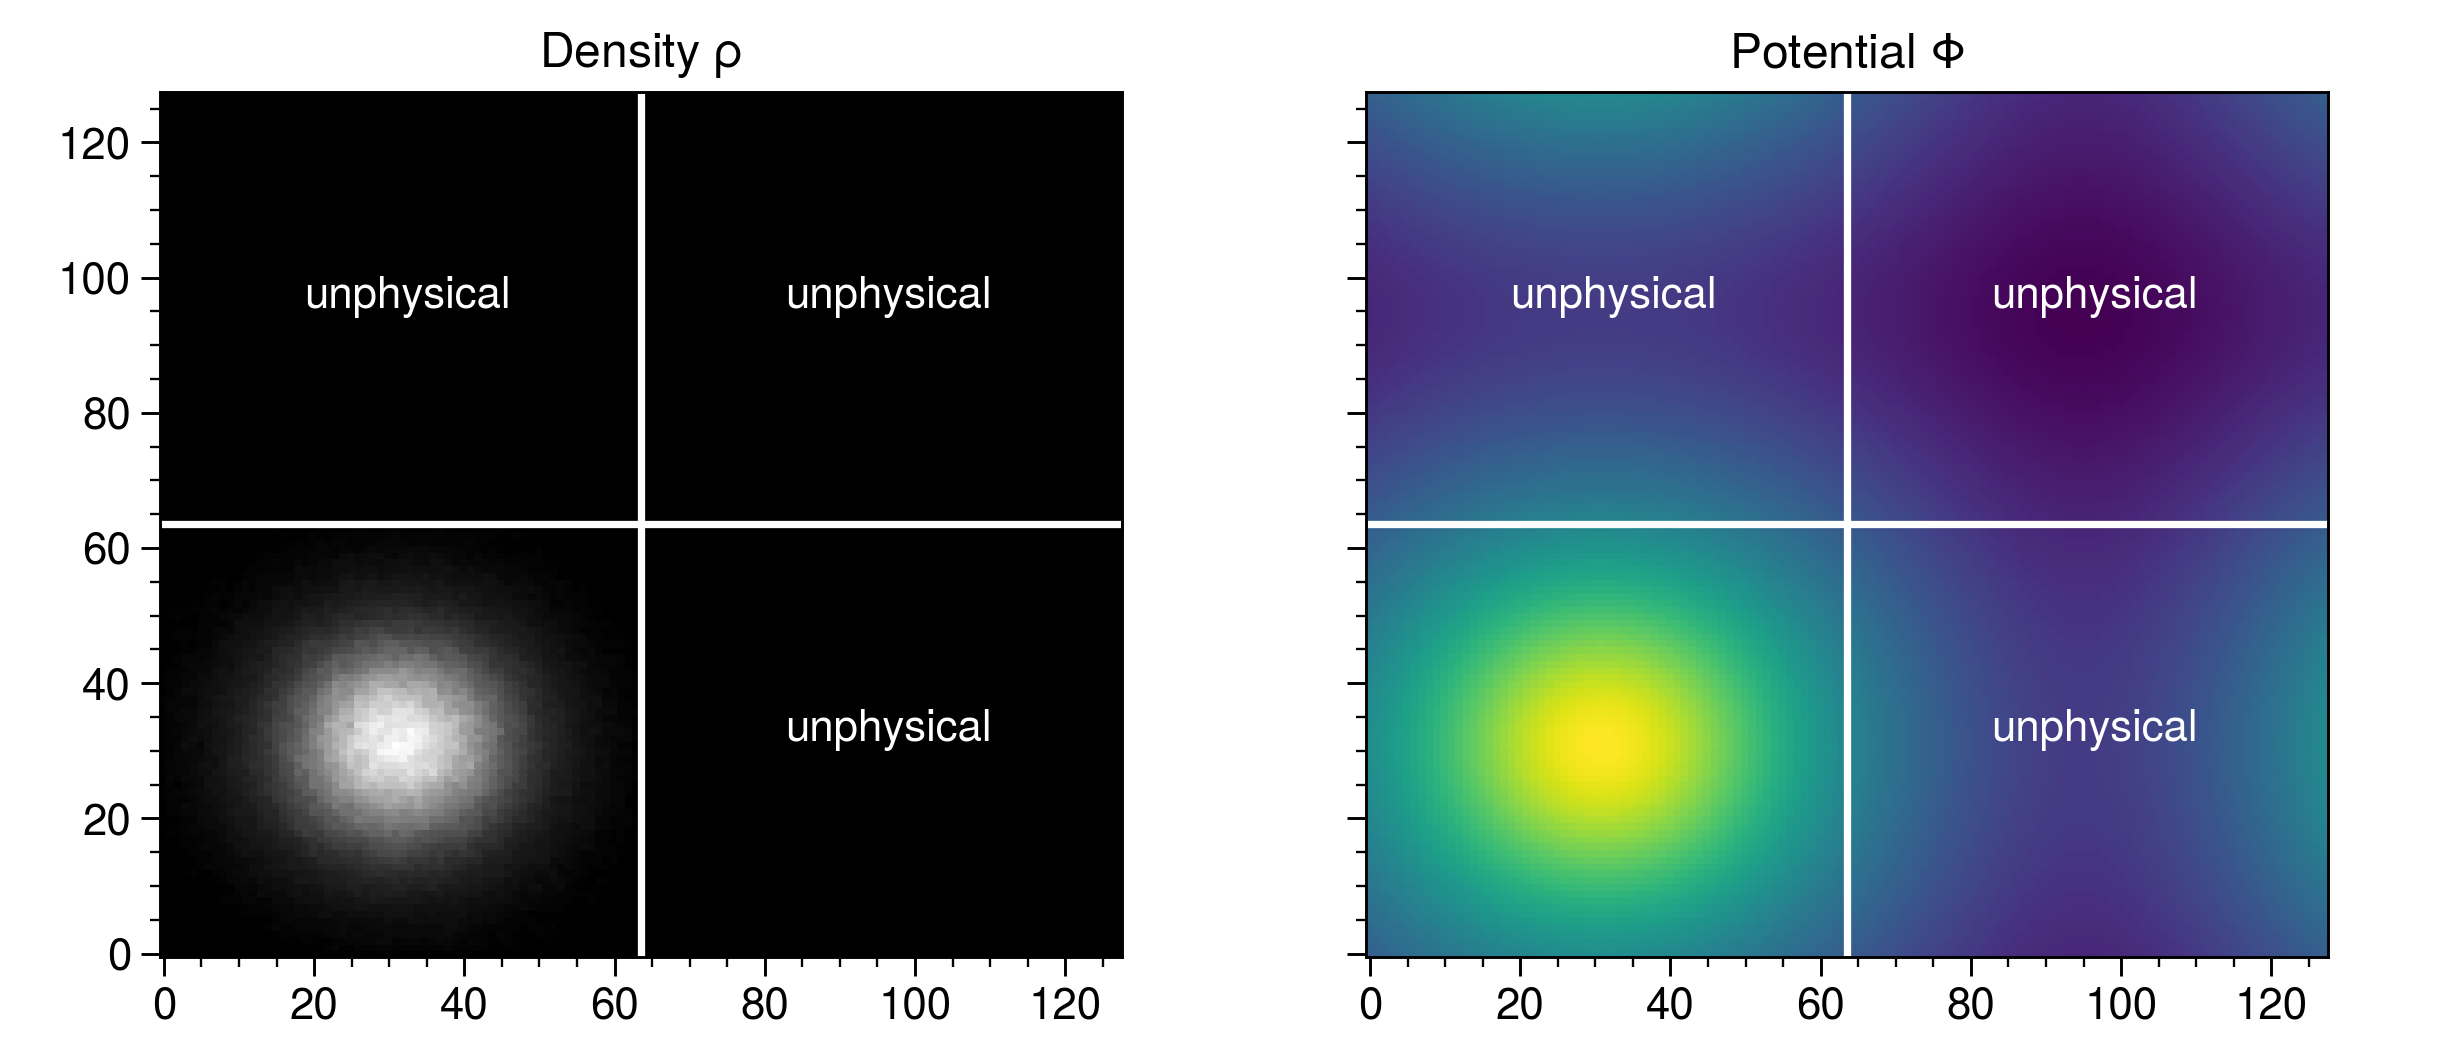
\includegraphics[width=\textwidth]{Images/chapter3/poisson.png}
    \caption{\label{fig:poisson}Solution of Poisson's equation on a doubled grid.}
    
\end{figure}
%

First, the charge density $\rho_{i,j}$ is obtained on a grid. A common method is to treat each macroparticle as a rectangular, uniform density cloud of charge with dimensions equal to the grid spacing, assigning a fractional charge to each bin according to the fraction of the cloud overlapping with that bin \cite{Birdsall1975}. Second, Poisson’s equation is solved on the grid. The method used in PyORBIT follows \cite{Hockney1981}. The potential is written as the convolution of a Green's function $G(\mathbf{x})$ with the charge density $\rho(\mathbf{x})$:
%
\begin{equation}
    \Phi(\mathbf{x}) = G(\mathbf{x}) * \rho(\mathbf{x}).
\end{equation}
%
We then exploit the convolution theorem \cite{Arfken1985} to write
%
\begin{equation}
    \mathcal{F}[\Phi(\mathbf{x})]
    =
    \mathcal{F}[G(\mathbf{x})] \cdot \mathcal{F}[\rho(\mathbf{x})]
\end{equation}
%
where $\mathcal{F}$ represents the Fourier transform. For a grid with $N$ bins per dimension, the time-complexity of the convolution is $O(N^2)$. The Fourier transform reduces this to $O(N \log N)$. To create periodic boundary conditions, the grid is doubled in each dimension. The Green's function is mirror-reflected onto these new regions, while the charge density is set to zero. The potential is solved for on the doubled grid, after which the unphysical regions are discarded. An example is shown in Fig.~\ref{fig:poisson}. Third, using the same weighting method as the first step, the gradient of the potential is interpolated at the particle positions. Finally, the particle momenta are updated using an appropriate integration scheme. 

In rings where the coasting beam approximation is valid, the longitudinal and transverse dimensions are treated separately. In PyORBIT, a longitudinal space charge node acts on the bunch once per turn. Two models are included for the transverse space charge calculation: the 2.5D model and the sliced model. In the 2.5D model, Poisson’s equation is solved once for a charge density obtained by projecting the entire bunch onto the $x$-$y$ plane; the transverse space charge forces are then weighted according to the longitudinal density. In the sliced model, the bunch is longitudinally sliced, and Poisson’s equation is solved for each slice.

In the discussion of space charge thus far, the beam was assumed to be in free space; in reality, the beam is in a conducting vacuum chamber. Charged particles leave so-called wake fields on the conducting surface, which then act on other particles or the same particle on subsequent turns, possibly leading to instability. The treatment of wake fields can be challenging and is introduced in \cite{Chao1993}. No details are described here; we only mention that PyORBIT takes these effects into account.



\subsection{Injection}

Injection is simulated by adding particles to the bunch at the foil location on each turn. Since each pulse is the sum of many minipulses from the linac, it is only necessary to use an approximate representation of the minipulse. A so-called JOHO distribution is used in the transverse plane, which resembles a truncated Gaussian. The design RMS emittance is approximately 0.3 mm~mrad. Recent measurements indicate that the emittance may be closer to 0.5 mm~mrad. Additionally, although the Twiss parameters are usually assumed to be matched to the ring ($\beta_x \approx \beta_y \approx 10$ m/rad, $\alpha_x \approx \alpha_y \approx 0$ rad), the measurements indicated that the $\beta$ functions may be closer to 4 m/rad and the alpha functions may be closer to -0.5. We use values close to these measurements. In the longitudinal plane, the spatial distribution is uniform and the energy distribution is a Gaussian with a mean of 1 GeV and a standard deviation of less than 1 MeV.

An important effect during charge-exchange injection is Coulomb scattering during passage through the stripper foil. This is handled by a foil scattering node that acts on the bunch at the foil position. This scattering process increases the effective emittance of the injected bunch.

Phase space painting can be simulated by adding an artificial time-dependent bump to the coordinates on each turn; however, it is more realistic to vary the strengths of the eight injection kickers in the model with the inclusion of element offsets from the closed orbit. The following procedure is used to set the coordinates at the injection point: Let $(x_o, x'_o, y_o, y'_o)$ be the desired coordinates. First, a particle is launched from the injection point with $x = x_o$, $x' = x'_o$, and $y = y' = 0$. The particle is tracked to the end of the injection region. An optimizer varies two kicker strengths to flatten the downstream orbit; i.e., obtain $x = x' = 0$ after tracking. Then, the particle is launched with $x = x_o$, $x' = -x'_o$ and tracked backwards to the start of the injection region. Two kickers are varied to flatten the upstream orbit; i.e., obtain $x = x' = 0$ at the start of the injection region. The process is repeated with the vertical orbit.


\subsection{Simulation procedure}

PyORBIT employs a two-language scheme: the core algorithms are written in C++ but are accessed at the Python level. All PyORBIT scripts are written in Python. The scripts used in this work are modified versions of previously benchmarked injection scripts.

For space charge calculations, a 128 $\times$ 128 $\times$ 64 grid is used with the sliced model. No more than 1 meter is allowed between solver nodes. The final number of particles is generally $5 \times 10^{5}$. With these settings, a 1000-turn injection simulation takes several days to run.

In all simulations, the turn-by-turn covariance matrix of the distribution at the injection point is saved to a file. If space permits, the turn-by-turn 6D phase space coordinates are saved to a single file as a multi-dimensional array of size $n T (T + 1) / 2 \times 6$, where $n$ is the number of macroparticles injected per turn and $T$ is the total number of turns. (The array is reshaped during analysis to obtain a $T$-element list of coordinate arrays.) Of course, the arrays can be saved only on certain turns. In addition to the injection point, the distribution is periodically saved at the entrance to the RTBT; it can be transported through the RTBT in a separate simulation.




\section{Fringe field compensation}

It is worth illuminating the finding from \cite{Holmes2018} that in an otherwise linear lattice, fringe fields tend to eliminate any cross-plane correlations in the beam when the tunes are near the difference resonance $\nu_x \approx \nu_y$. To demonstrate this, a Danilov distribution matched to a linearized version of the SNS ring was generated. Fringe fields were then turned on, and the particles were tracked without space charge. Fig.~\ref{fig:fringe_a} shows the turn-by-turn evolution of the distribution.

\begin{figure}[!p]
    \centering
    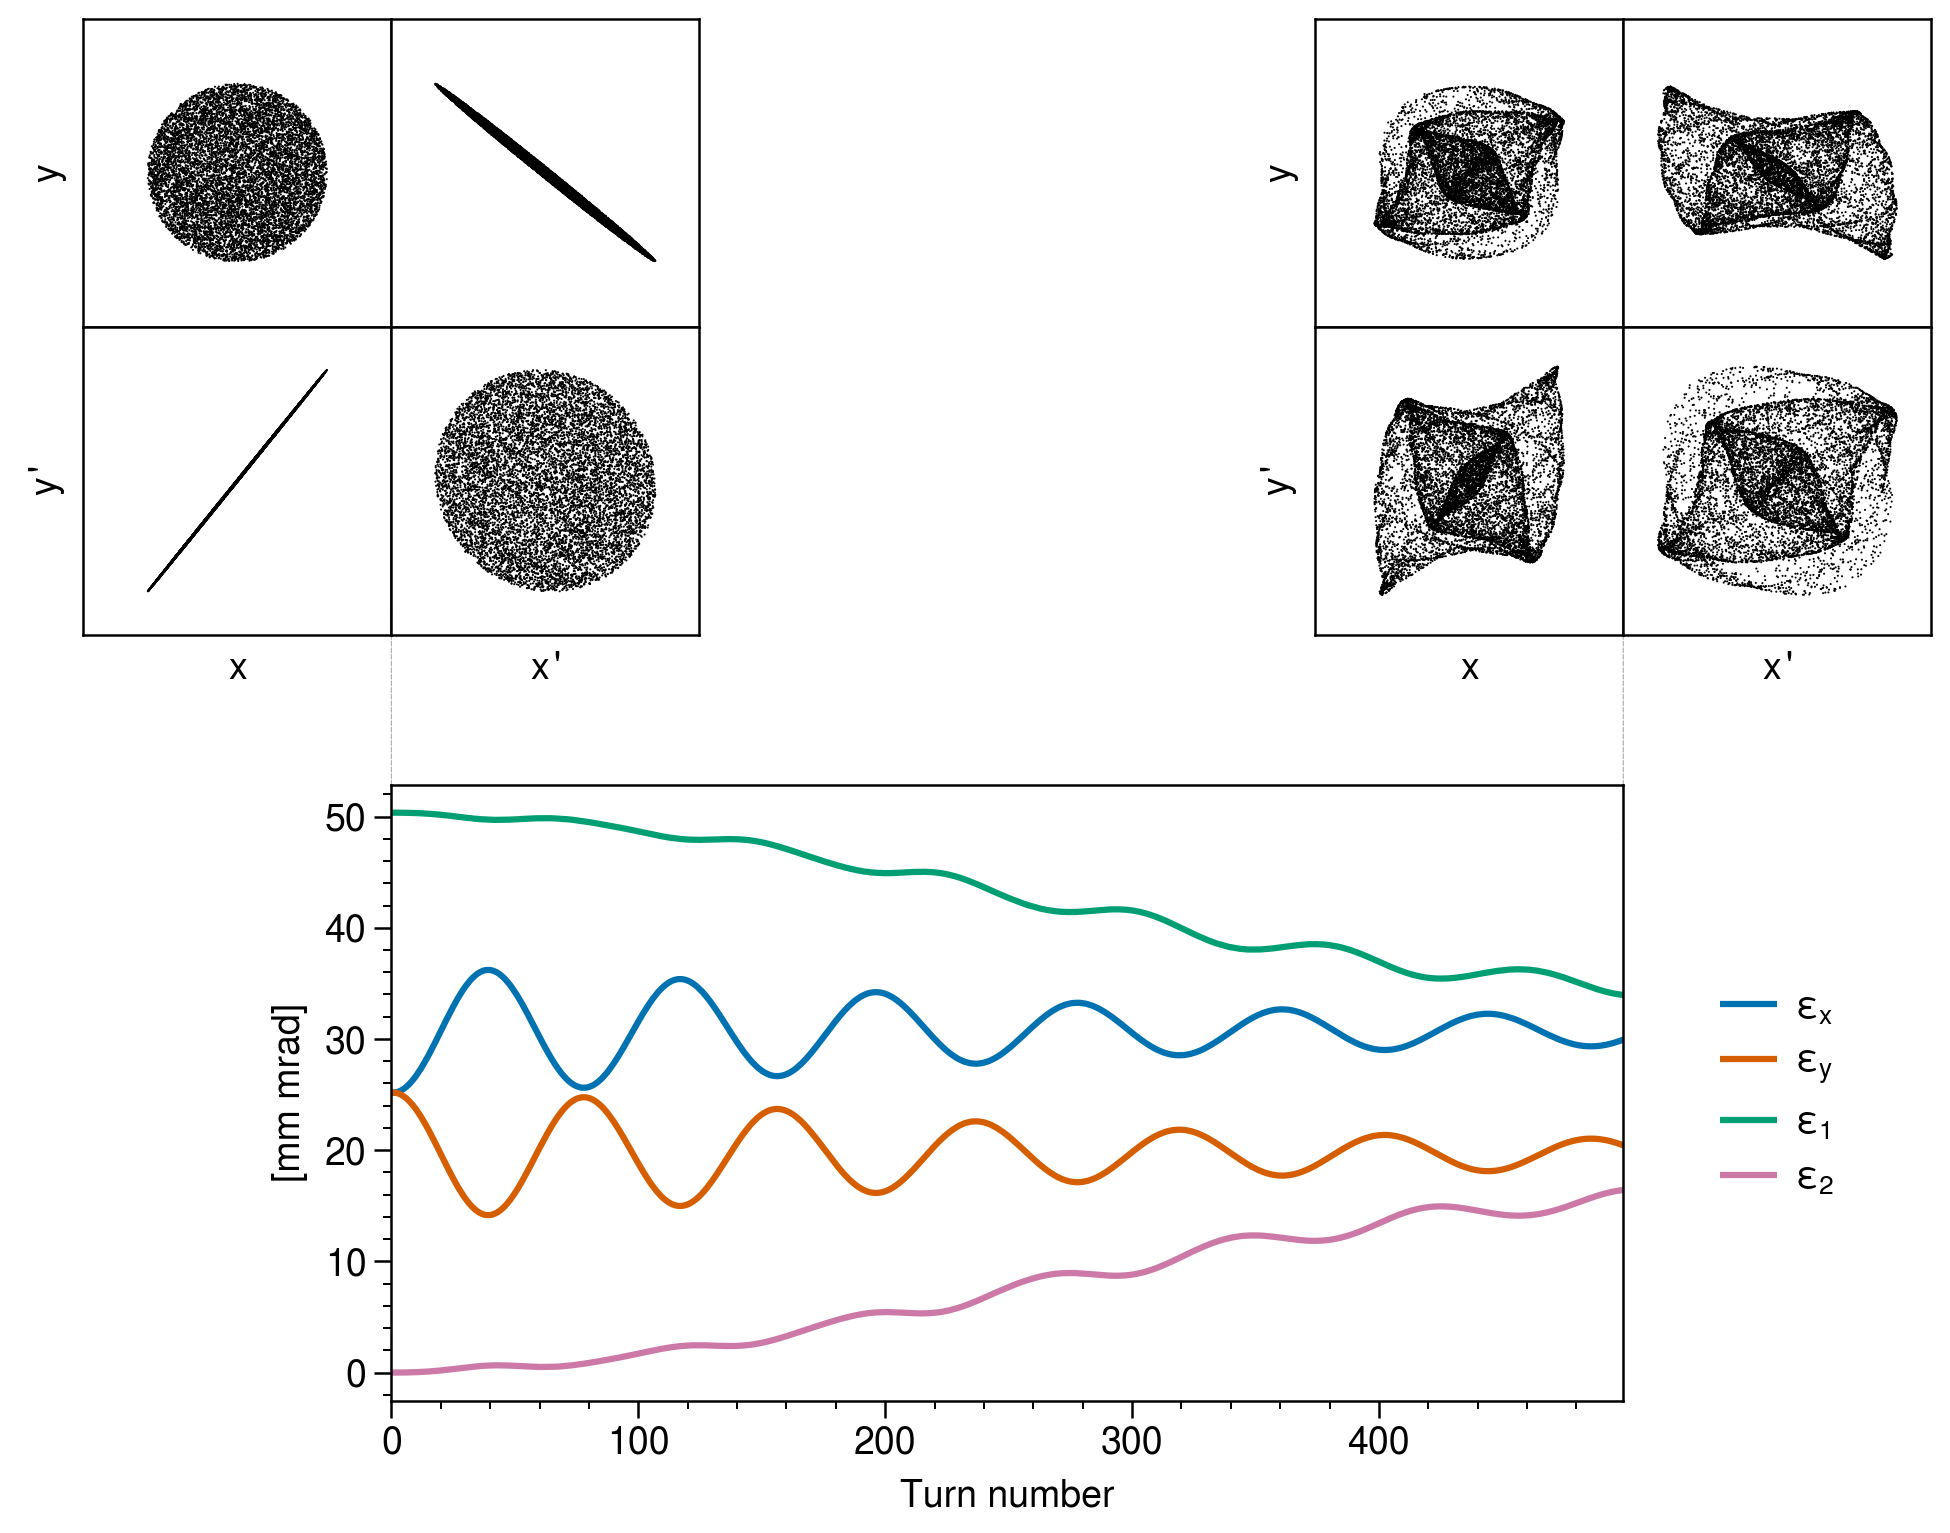
\includegraphics[width=0.7\textwidth]{Images/chapter3/fringe.png}
    \caption{Danilov distribution tracked in the SNS ring. Fringe fields are the only nonlinear external effect.}
    \label{fig:fringe_a}
    \vspace*{3cm}
\end{figure}

\begin{figure}[!p]
    \centering
    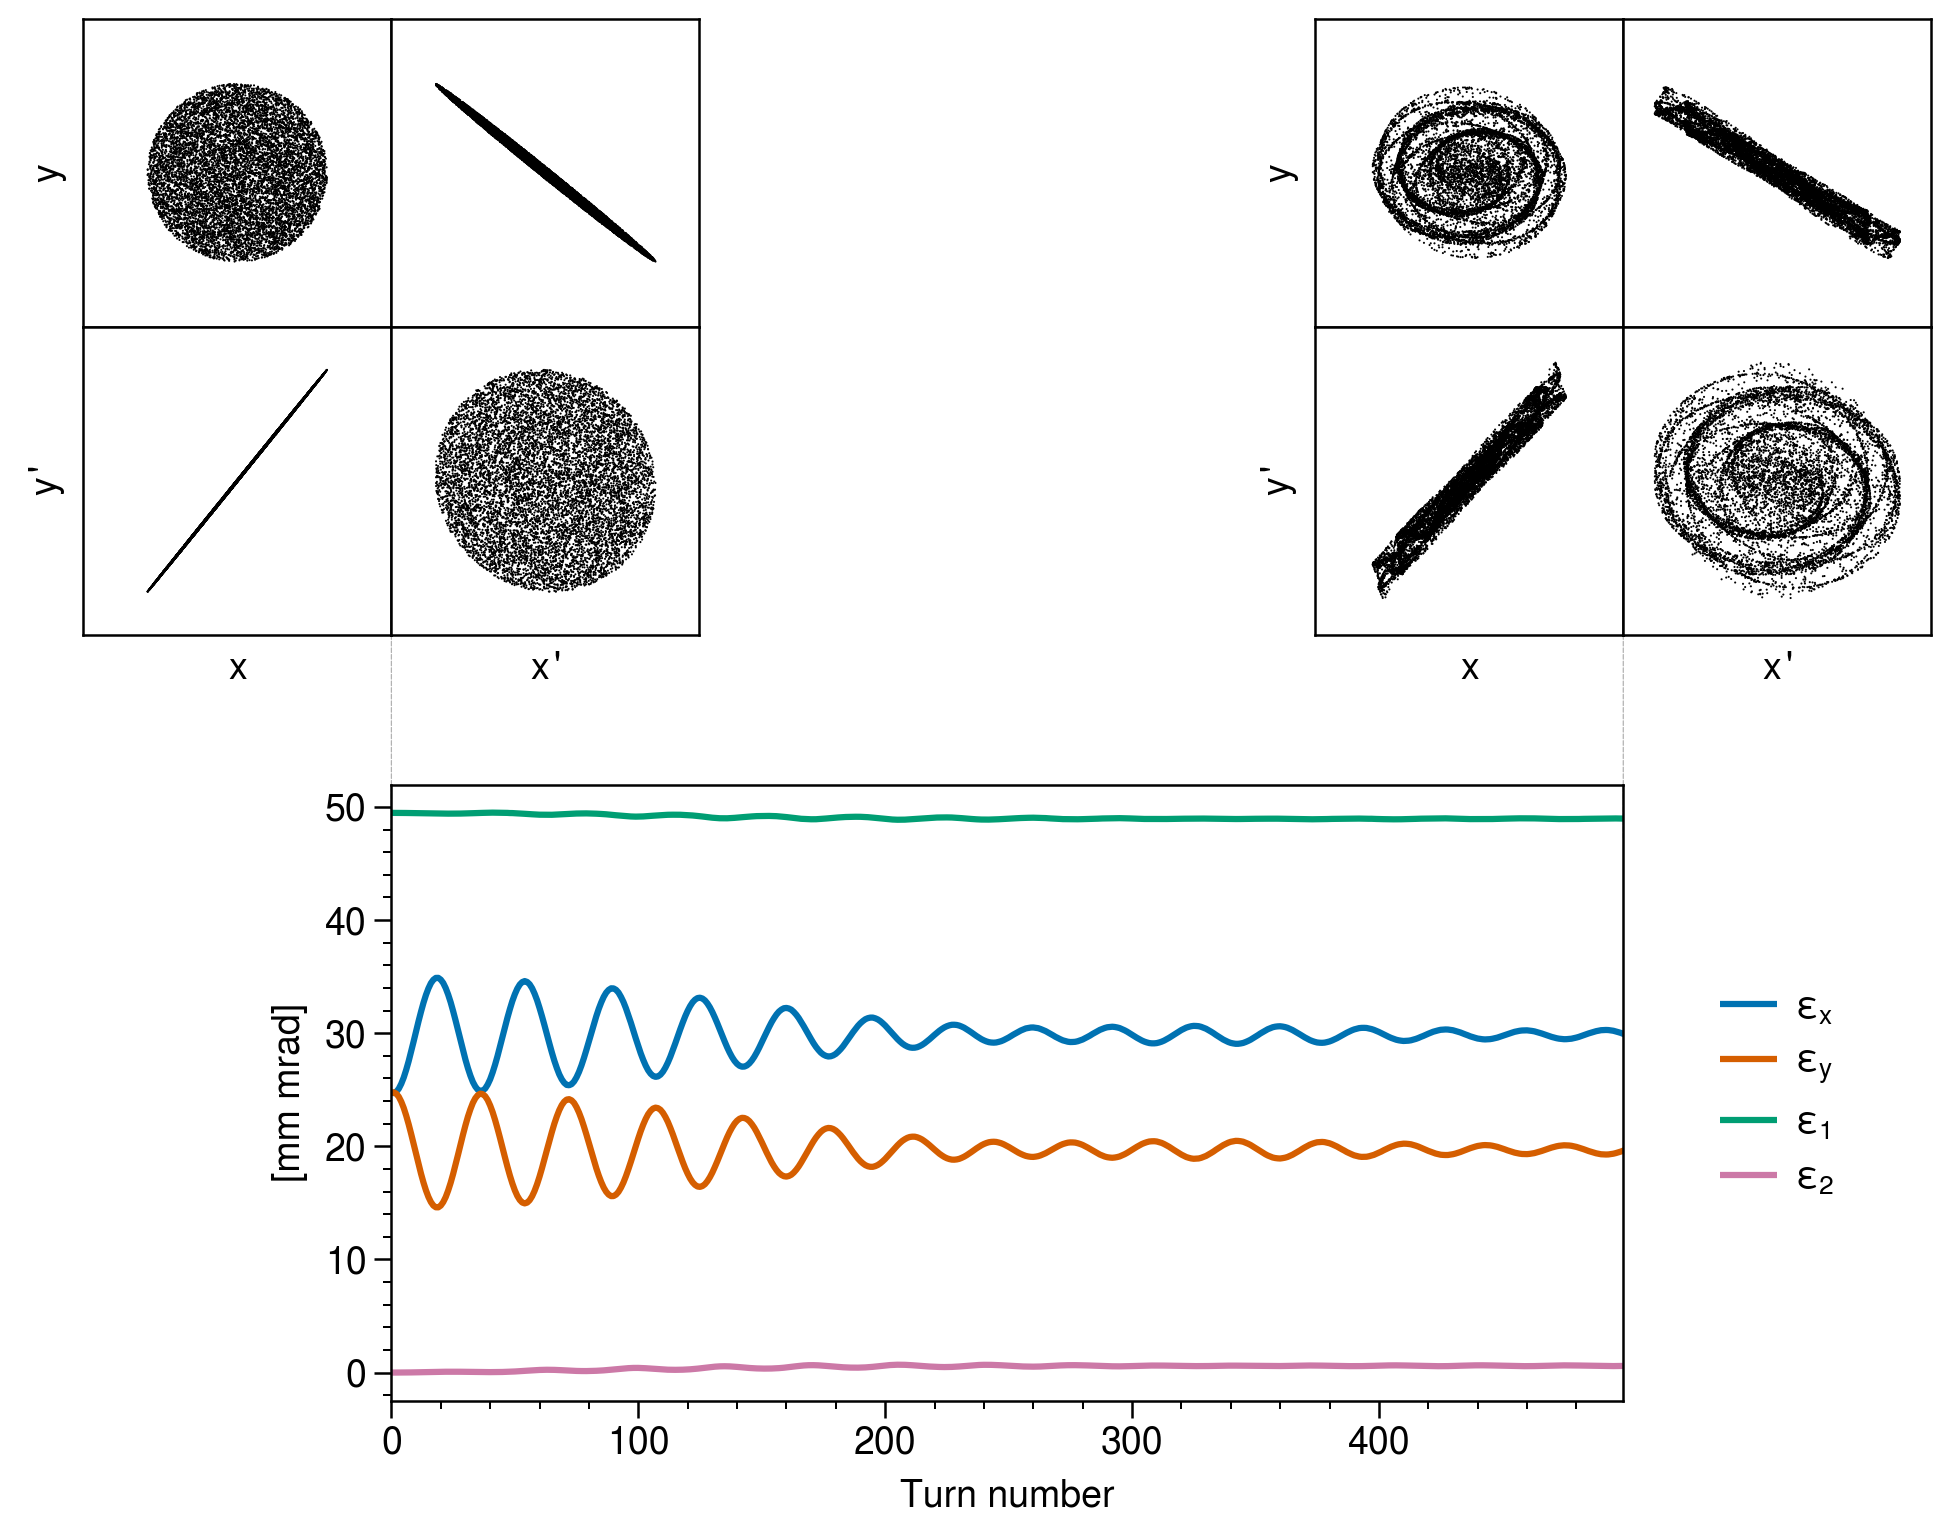
\includegraphics[width=0.7\textwidth]{Images/chapter3/fringe_solenoid.png}
    \caption{Danilov distribution tracked in the SNS ring with a solenoid added to the ring. Fringe fields are the only nonlinear external effect.}
    \label{fig:fringe_b}
    \vspace*{3cm}
\end{figure}

\begin{figure}[!p]
    \centering
    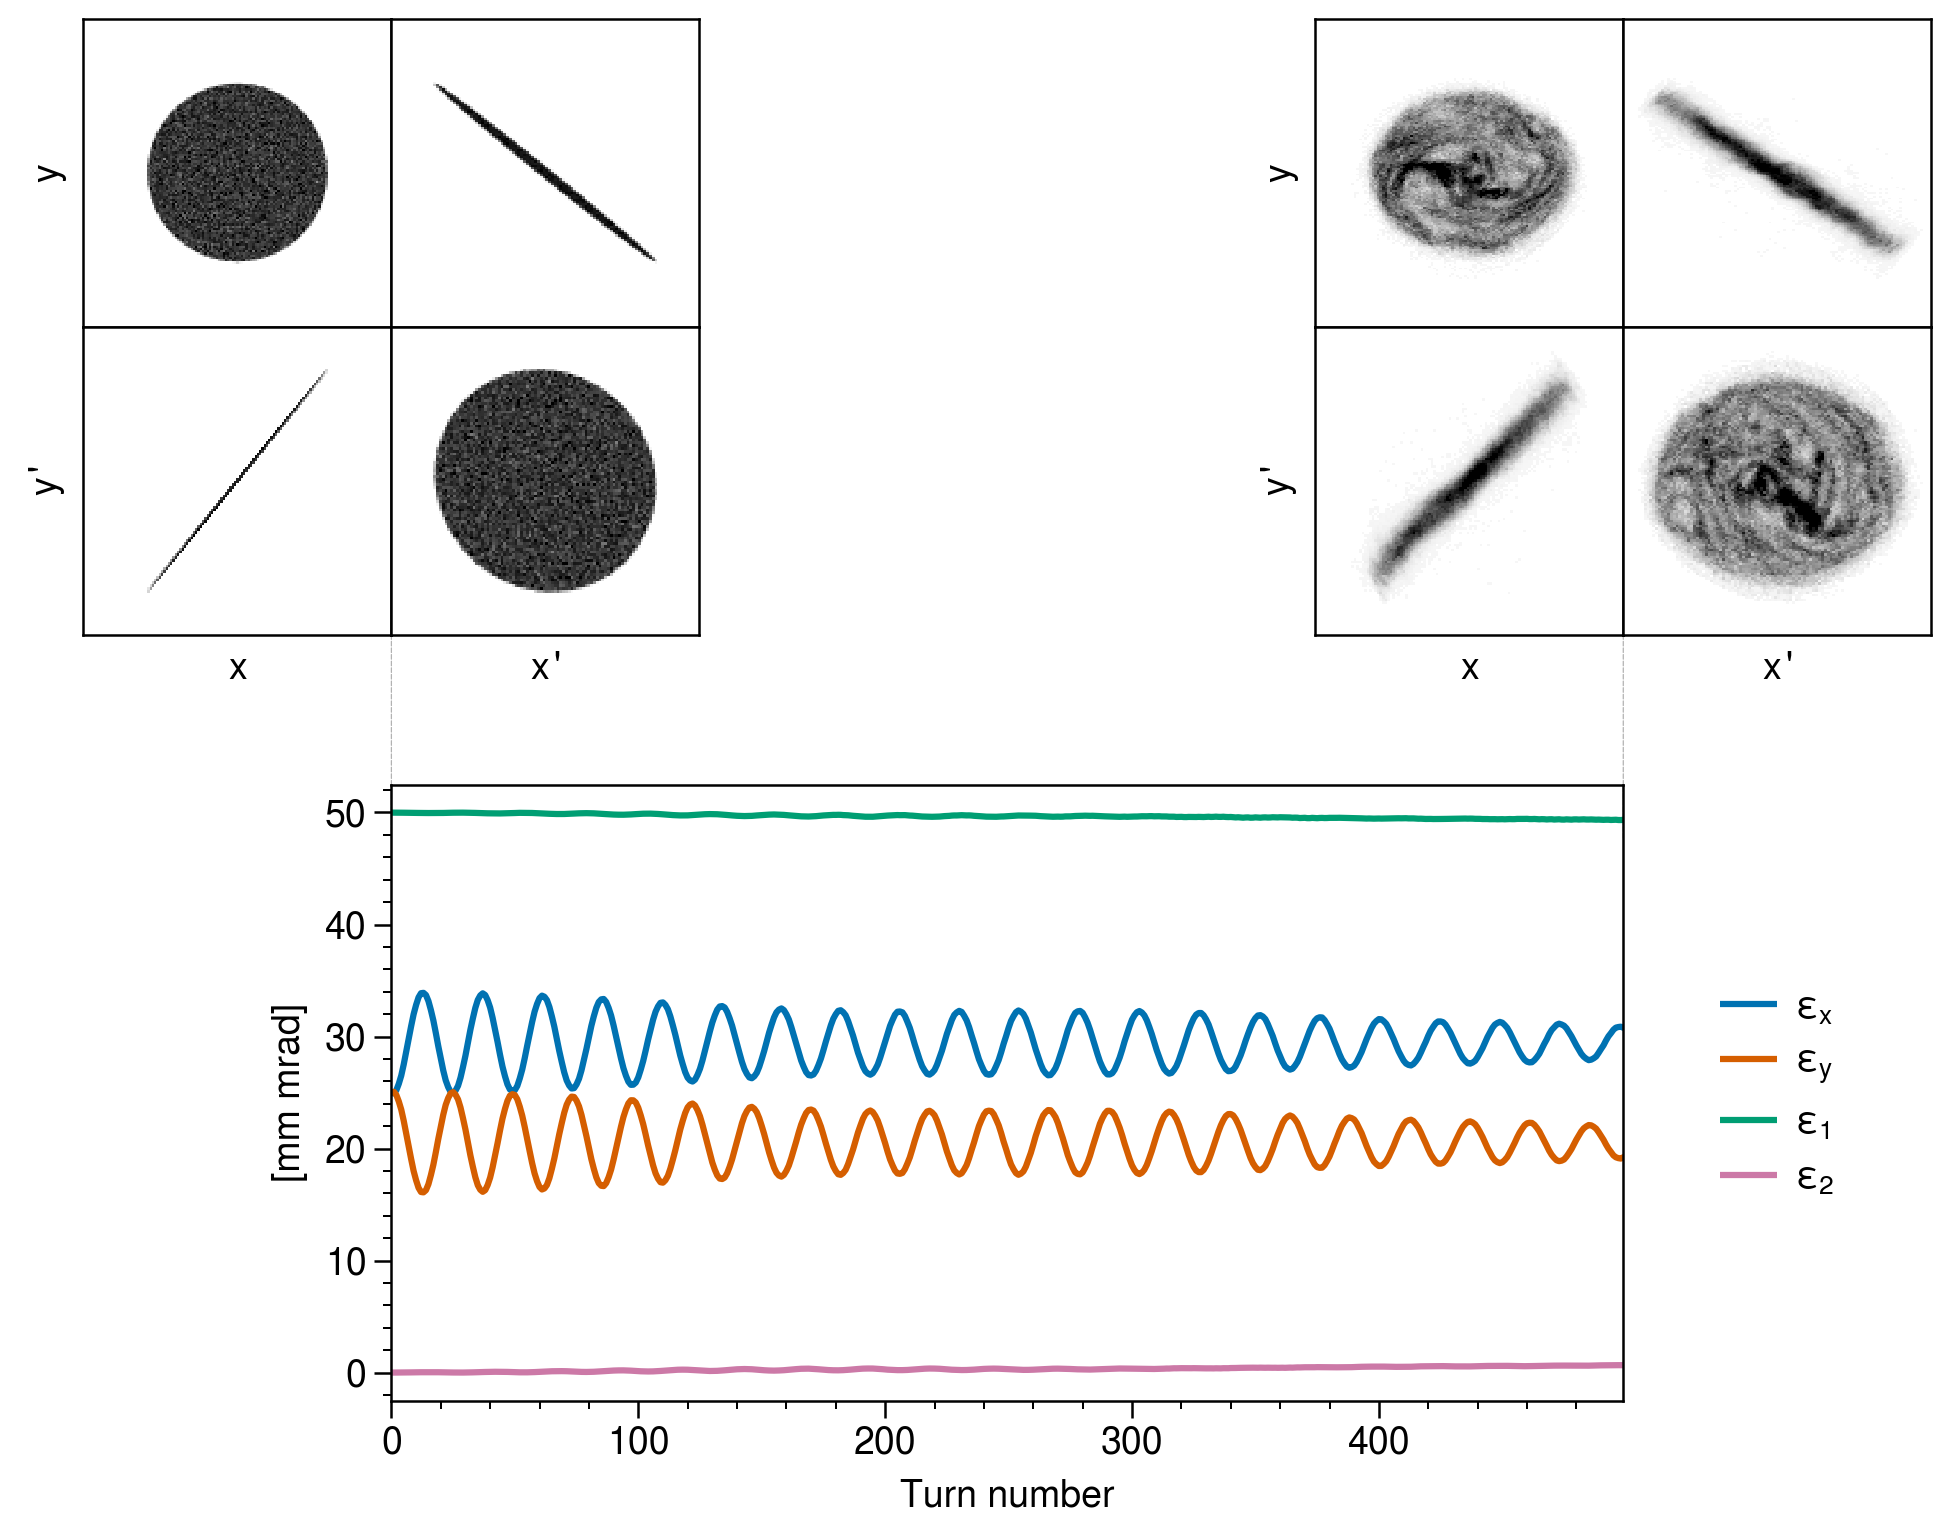
\includegraphics[width=0.7\textwidth]{Images/chapter3/fringe_spacecharge.png}
    \caption{Danilov distribution tracked in the SNS ring with space charge. Fringe fields are the only nonlinear external effect.}
    \label{fig:fringe_c}
    \vspace*{3cm}
\end{figure}


There is nonlinear coupling between the horizontal and vertical motion, and the final distribution is a superposition of rotating and counter-rotating modes. In Fig.~\ref{fig:fringe_b}, a solenoid magnet is added to the ring. The cross-plane correlations are now mostly maintained. The tunes $\nu_{1, 2}$ are no longer equal due to the linear coupling from the solenoid, so the resonance condition is avoided. In Fig.~\ref{fig:fringe_c}, the simulation is repeated with the inclusion of space charge instead of the solenoid magnet. An intensity of $10^{14}$ is used and the bunch length is equal to the ring length. It appears that a Danilov distribution will self-stabilize against the difference resonance when space charge is included.

It is recommended, however, that solenoid magnets be added to the ring to carry out this painting scheme. The difficulty is that the fringe fields dominate at the beginning of injection, when the transverse displacement is maximum, before space charge has a chance to stabilize the beam. This will be evident in several of the following simulations.



\section{Painting simulations}


\subsection{Best-case scenario}

The final simulation in \cite{Holmes2018} produced an approximate Danilov distribution. Only the final 1D projections of the distribution were displayed in the publication, and the intrinsic emittances were not calculated, so it is worth revisiting this simulation. Projections of the final distribution are shown in Fig.~\ref{fig:Holmes_corner_compare}.
%
\begin{figure}[!p]
    \centering
    \begin{subfigure}{0.8\textwidth}
        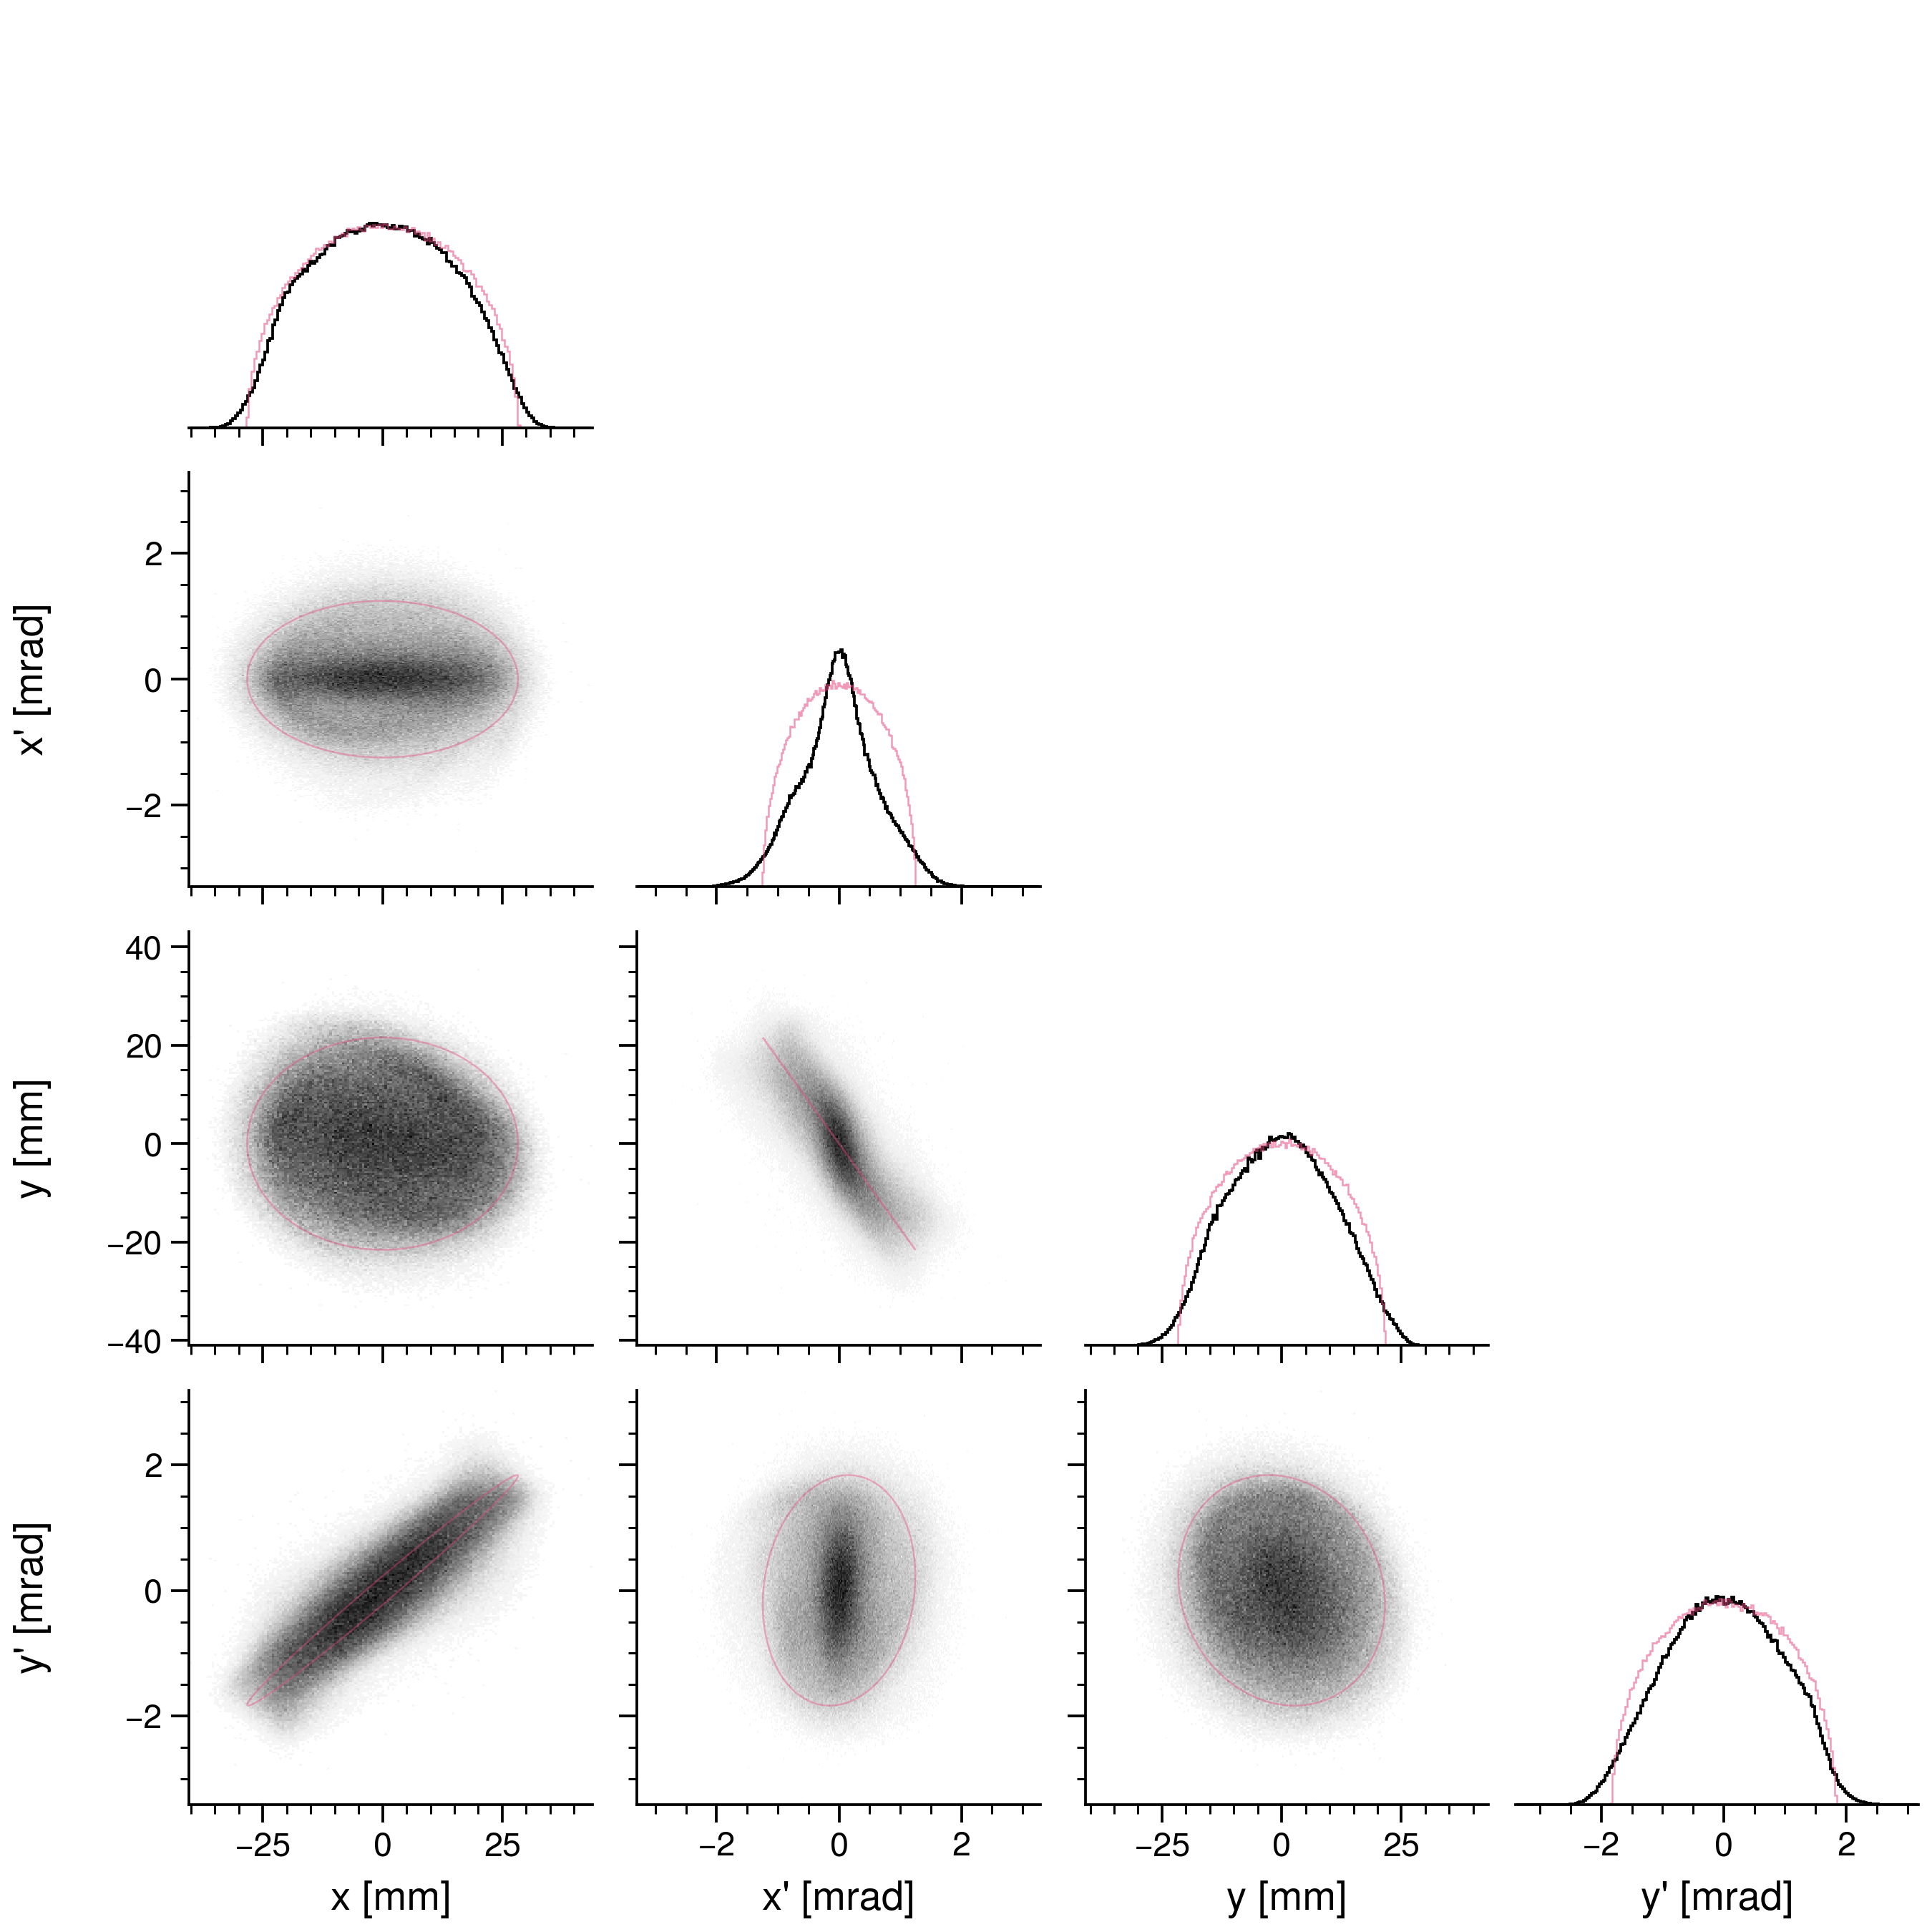
\includegraphics[width=\textwidth]{Images/chapter3/Holmes_corner_compare.png}
        \caption{1D and 2D projections of the final distribution at the injection point. The faint lines show the projections of an ideal Danilov distribution with the same Twiss parameters and apparent emittances as the simulated distribution.}
        \label{fig:Holmes_corner_compare}
    \end{subfigure}
    \vfill
    \vspace*{1.25cm}
    \vfill
    \begin{subfigure}{0.5\textwidth}
        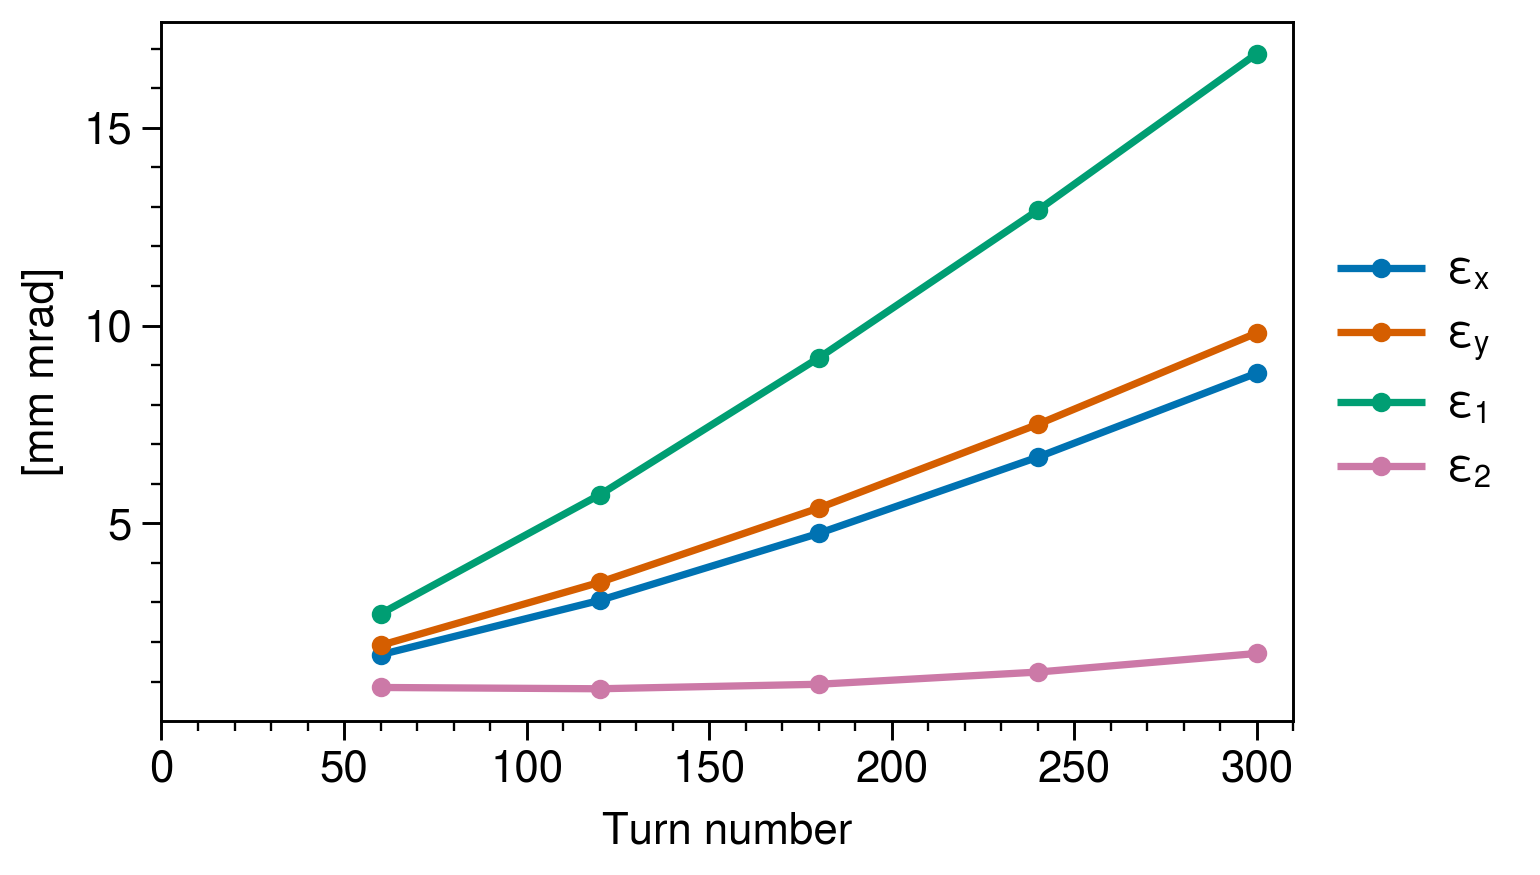
\includegraphics[width=\textwidth]{Images/chapter3/Holmes_emittances.png}
        \caption{RMS emittances every 60 turns during injection.}
        \label{fig:Holmes_emittances}
    \end{subfigure}
    \caption{Distribution from the final simulation in \cite{Holmes2018}.}
\end{figure}
%
The faint pink lines represent the projections of an ideal Danilov distribution with the same Twiss parameters and apparent emittances as the simulated distribution. Although the 1D projections have developed tails, they are relatively close to the ideal case. The exception is the $x'$ projection, which has developed a sharp peak. The 2D projections are also not too far from ideal. Although the $x$-$y'$ and $y-x'$ projections have been broadened, they exhibit the correct correlations. And the beam is round in the $x$-$y$ plane. Fig.~\ref{fig:Holmes_emittances} shows that the smaller intrinsic emittance remains close to its lower limit throughout injection. 

Several steps were necessary to achieve this simulated result. First, the painting path was chosen to follow a line in the $x$-$y'$ plane. The apparent emittances were kept somewhat equal. Both these steps were discussed in chapter \ref{chap-2}. Third, the ring RF cavity voltages were decreased to better approximate a coasting beam. Fourth, the beam energy was lowered to 0.6 GeV to increase the effective kicker strength; additionally, orbit corrector dipoles in the injection region provided a closed vertical bump. These modifications allowed a vertical slope of 1.58 mrad at the injection point. Fifth, the number of injected turns was reduced from 1000 to 300 to compensate for the increased space charge strength at the lower energy. Finally, a solenoid magnet was added to the ring to mitigate the effect of fringe fields. 

This is likely the best-case scenario in the SNS. But as will be discussed in chapter \ref{chap-5}, new experimental constraints have come to light. The SNS cannot reach 0.6 GeV, and the use of orbit correctors in the injection region is difficult. The net result is that the maximum vertical slope is limited and that space charge will be less intense. Additionally, the minipulse may be significantly mismatched at the injection point. Finally, a solenoid magnet will not be present during initial experiments in the SNS. The effect of these constraints should be examined with simulation.

[Elliptical painting is carried out in the SNS in chapter \ref{chap-5}. After several of these experiments, a simulation will be shown for comparison. For now, [...]]
[Some things we might show in this chapter:
\begin{itemize}
    \item No solenoid
    \item Unequal emittances
    \item Bipolar kickers]
\end{itemize}


% \begin{figure}[!p]
%     \centering
%     \begin{subfigure}{\textwidth}
%         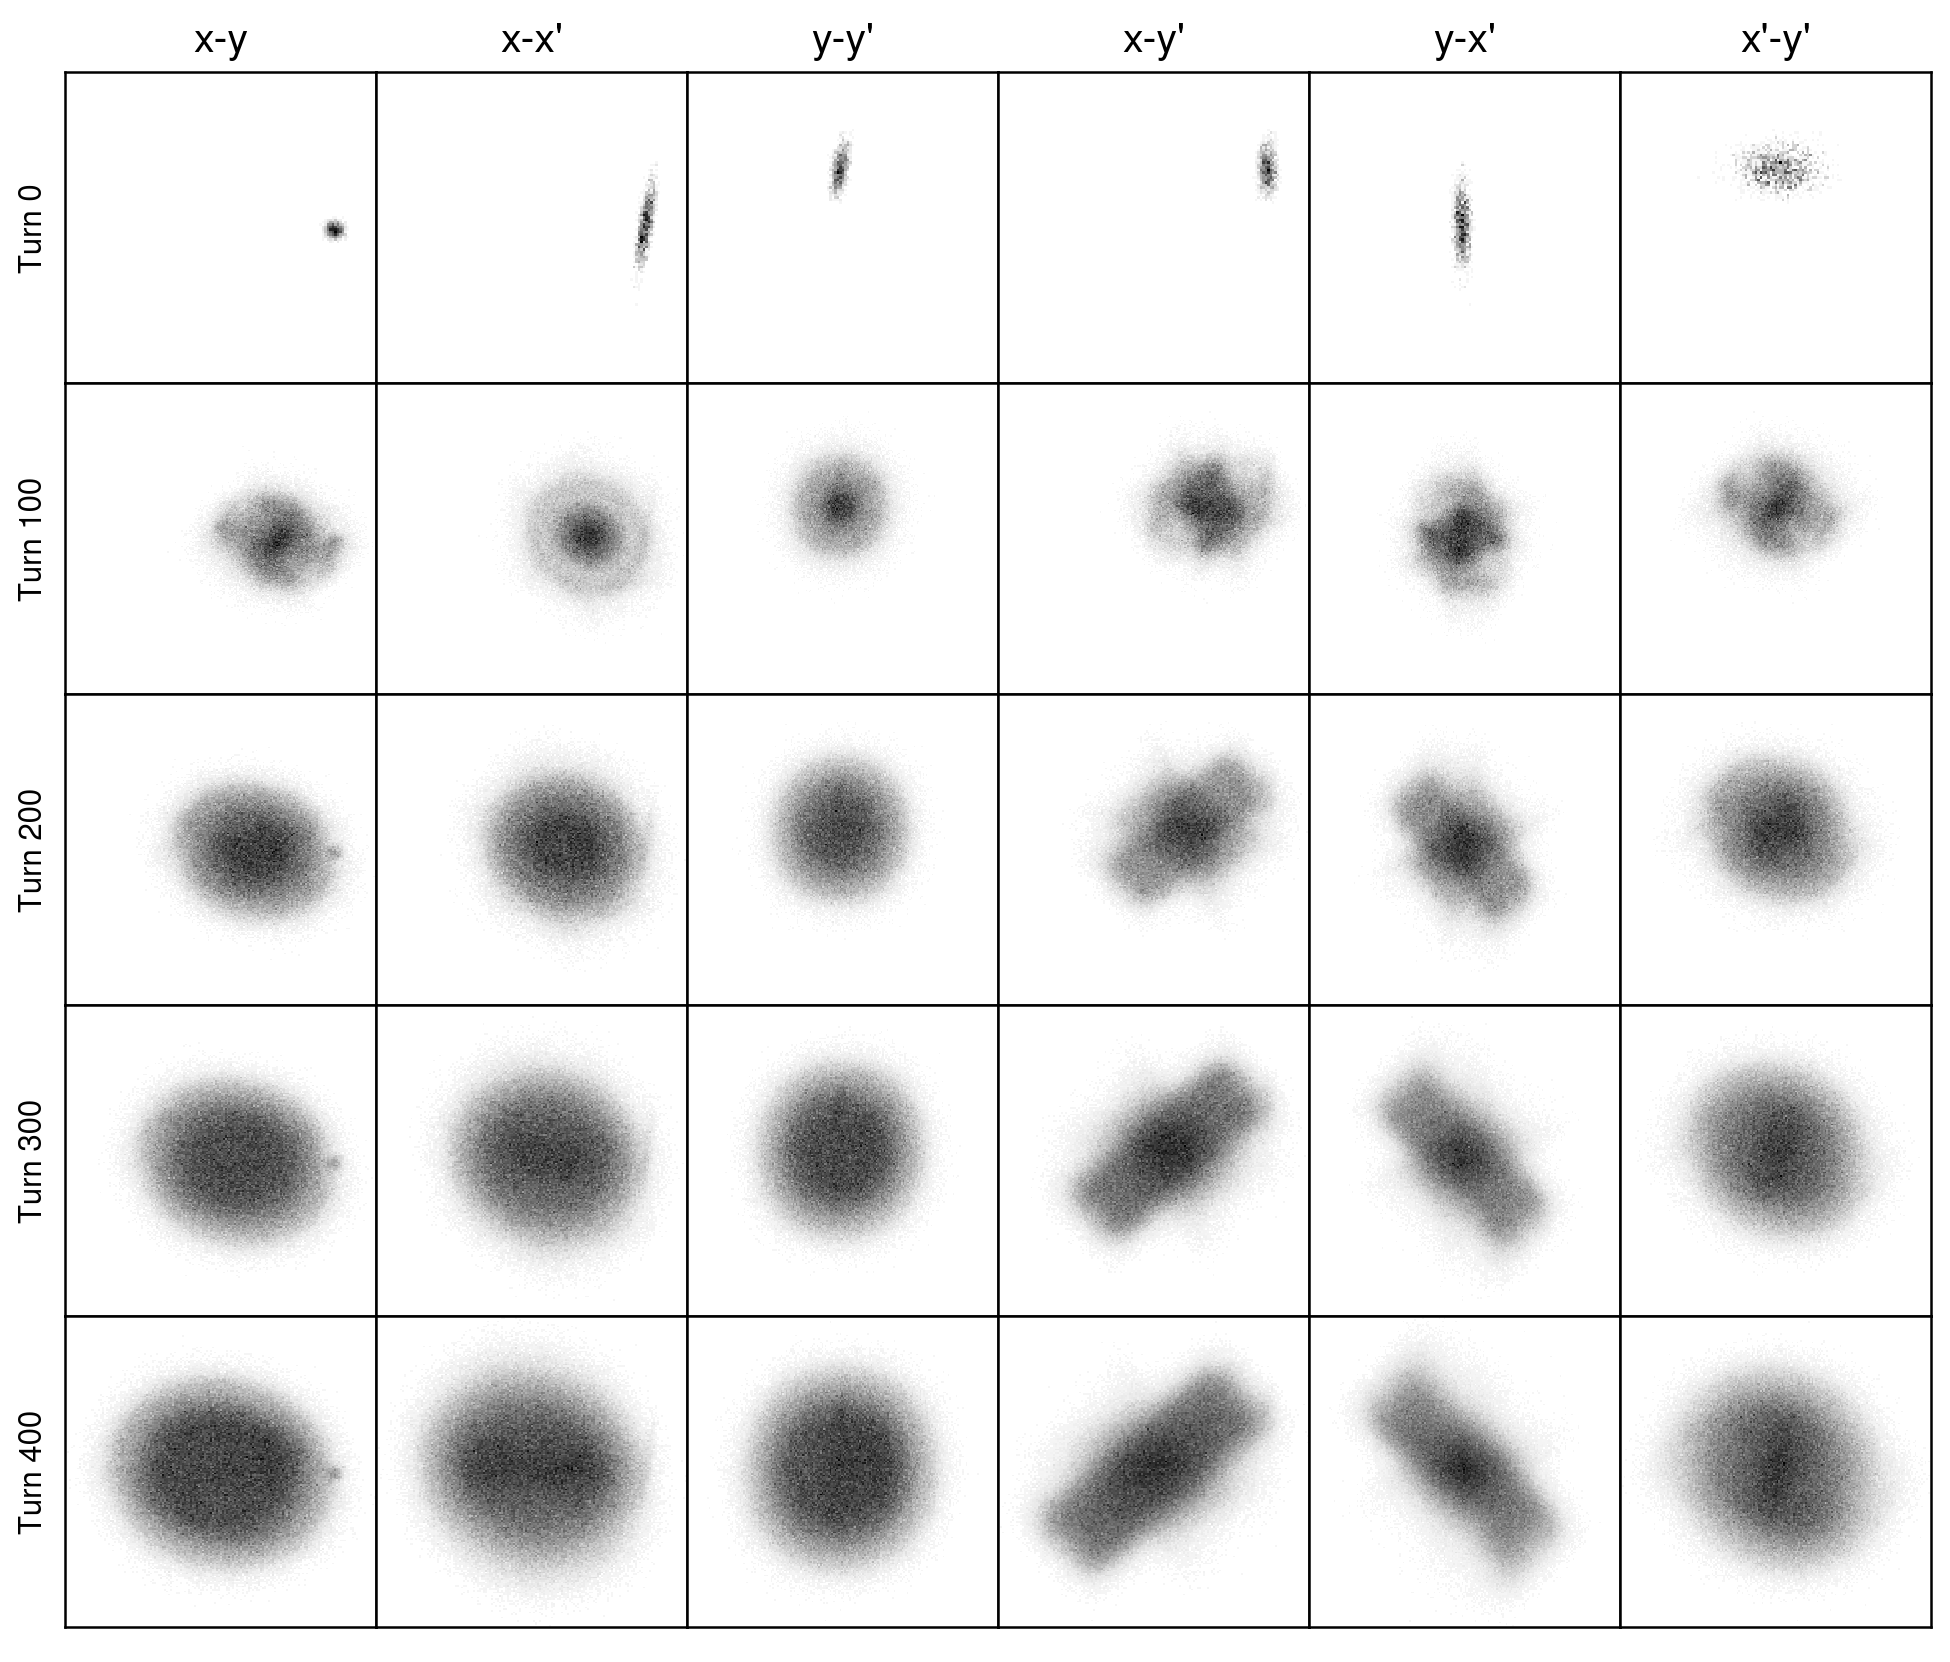
\includegraphics[width=\textwidth]{Images/chapter3/snapshots.png}
%     \end{subfigure}
%     \vfill
%     \vspace*{1.0cm}
%     \vfill
%     \begin{subfigure}{0.7\textwidth}
%         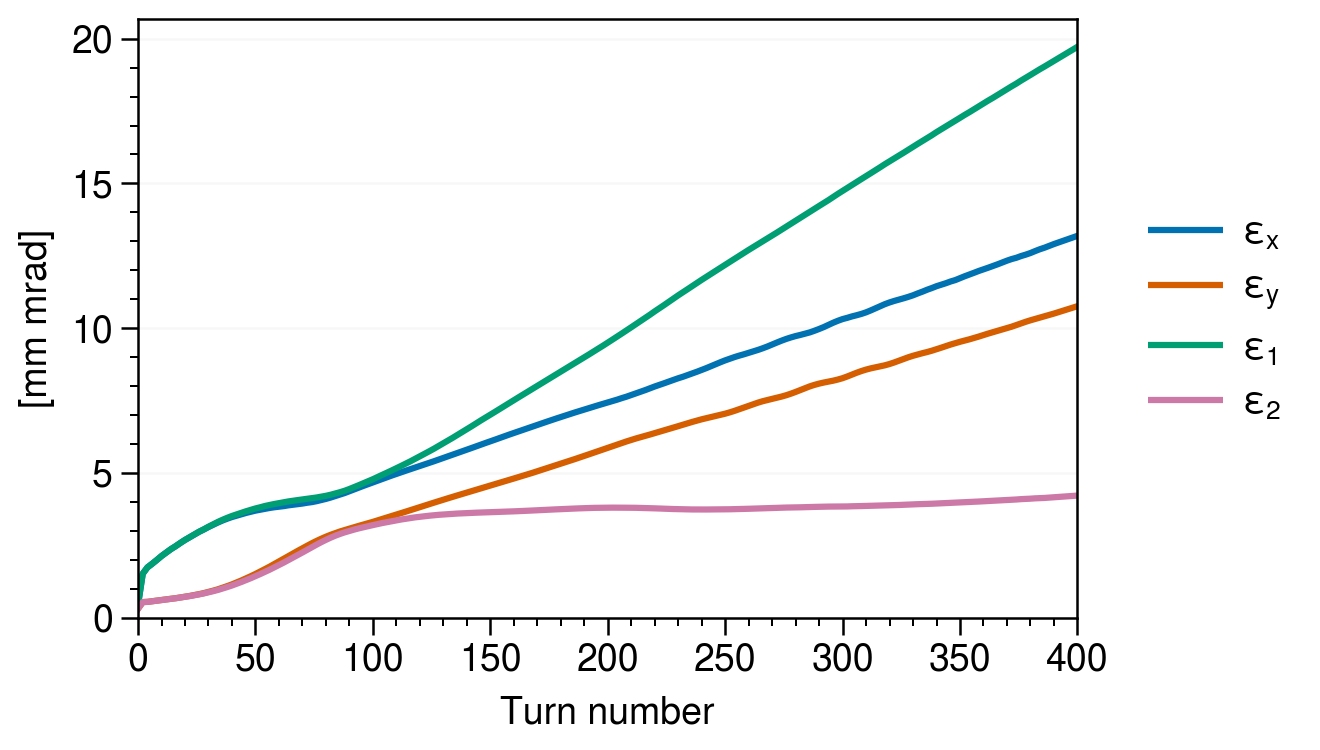
\includegraphics[width=\textwidth]{Images/chapter3/emittances.png}
%     \end{subfigure}
%     \caption{Simulation of elliptical painting.}
%     \label{fig:my_label}
% \end{figure}
